\section{Membuat Halaman Baru Jika Sudah Membuat Halaman Master saat Membuat Aplikasi App Builder}
Berikut cara membuat page baru jika sudah membuat page master , kita akan membuat page ORMAWA,JURUSAN,dan JABATAN\_ORMAWA, kita salah satukan contoh pada ORMAWA.
        \begin{itemize}
        \begin{figure}
        \item[1]Kita Kembali Ke Nomer 18 lalu Pilih Create Page Untuk Membuat Page DATA ORMAWA dan FORM ORMAWA
        \begin{center}
        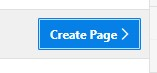
\includegraphics[scale=0.9]{figures/buat_page_baru.jpg}
        \caption{\textit{Create Page}}
        \end{center}
        \end{figure}
        
        \begin{figure}[!htbp]
        \item[2]Lalu Kita Pilih Report Lali Klik Next
        \begin{center}
        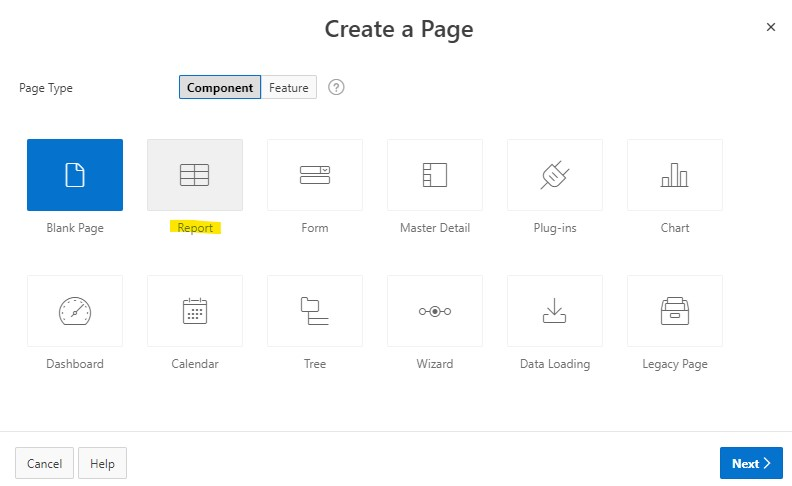
\includegraphics[scale=0.5]{figures/pilih_report.jpg}
        \caption{\textit{Memilih Report}}
        \end{center}
        \end{figure}
        
        \begin{figure}[!htbp]
        \item[3]Pilih Report With Form
        \begin{center}
        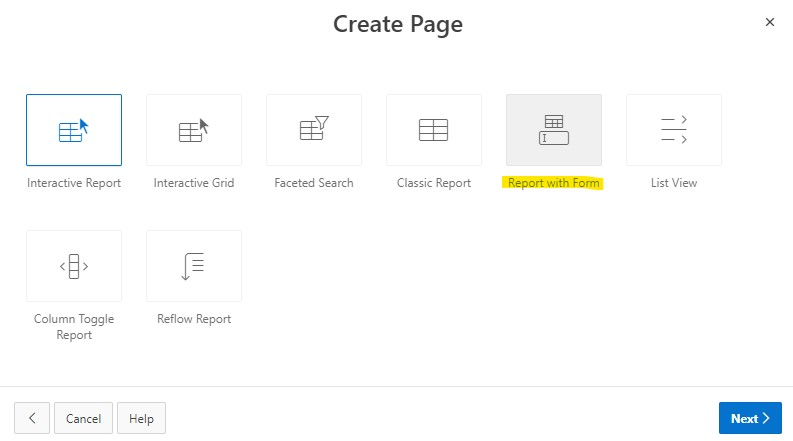
\includegraphics[scale=0.5]{figures/pilih_report_with_form.jpg}
        \caption{\textit{Pilih Report With Form}}
        \end{center}
        \end{figure}
        
        \begin{figure}[!htbp]
        \item[4]Lalu Isi Report Page Name dan Form Page Name Seperti Berikut , abaikan yang lain lalu klik next
        \begin{center}
        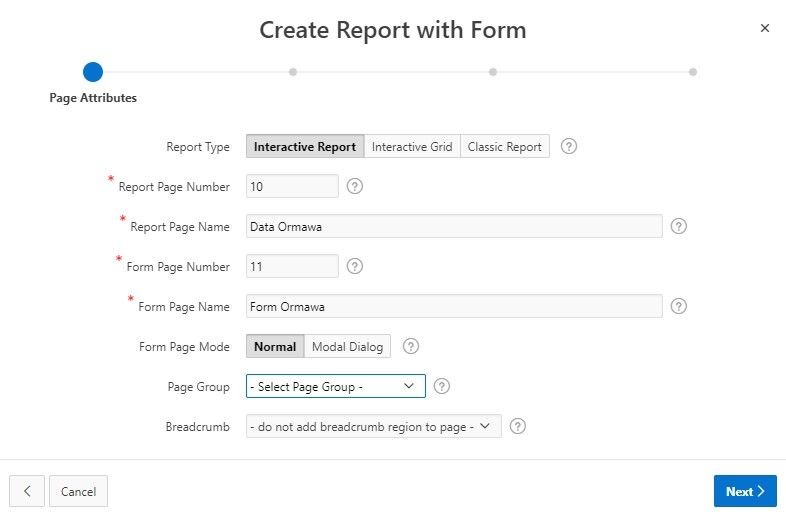
\includegraphics[scale=0.5]{figures/isi_sesuai_kebutuhan_tabel_dan_form_yg_akan_digunakan.jpg}
        \caption{\textit{Create Report With Form}}
        \end{center}
        \end{figure}
        
        \begin{figure}[!htbp]
        \item[5]Lalu pilih Create a new navigation menu entry lalu masukkan pada navigasi mahasiswa
        \begin{center}
        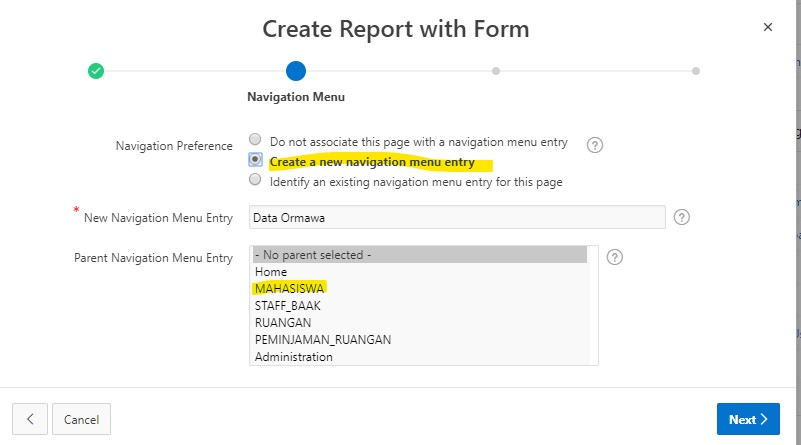
\includegraphics[scale=0.5]{figures/pilih_yang_ditandai.jpg}
        \caption{\textit{Masukan Navigasi}}
        \end{center}
        \end{figure}
        
        \begin{figure}[!htbp]
        \item[6]Pilih Table/View Name isikan tabel Ormawa Yang Telah Dibuat Tadi Lalu Klik Next dan Next Lagi
        \begin{center}
        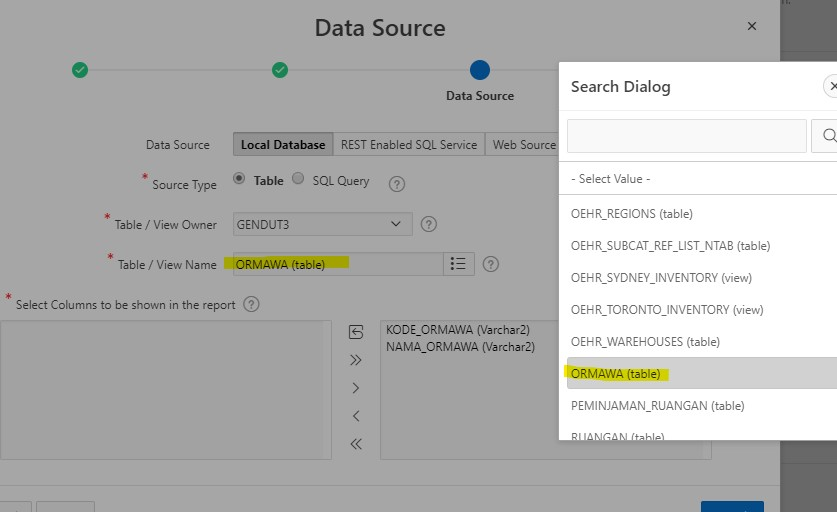
\includegraphics[scale=0.47]{figures/pilih_tabel_ormawa_yg_sudah_dibuat.jpg}
        \caption{\textit{Memilih Tabel Ormawa Dimasukkan pada Page Report Baru}}
        \end{center}
        \end{figure}
        
        \begin{figure}[!htbp]
        \item[7]Setelah terbuat ada 2 Page Ormawa yaitu Data(Untuk Menampilkan Tabel) dan Form Ormawa(untuk menampilakn isian form yang nanti akan diisi ke data tabel), Pertama kita lihat ke Data Ormawa
        \begin{center}
        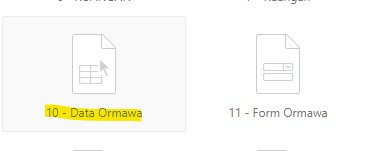
\includegraphics[scale=0.45]{figures/kita_pilih_terlebih_dahulu_data_ormawa.jpg}
        \caption{\textit{Page ORMAWA}}
        \end{center}
        \end{figure}
        
        \begin{figure}[!htbp]
        \item[8]Berikut adalah Halaman Edit Page Designer
        \begin{center}
        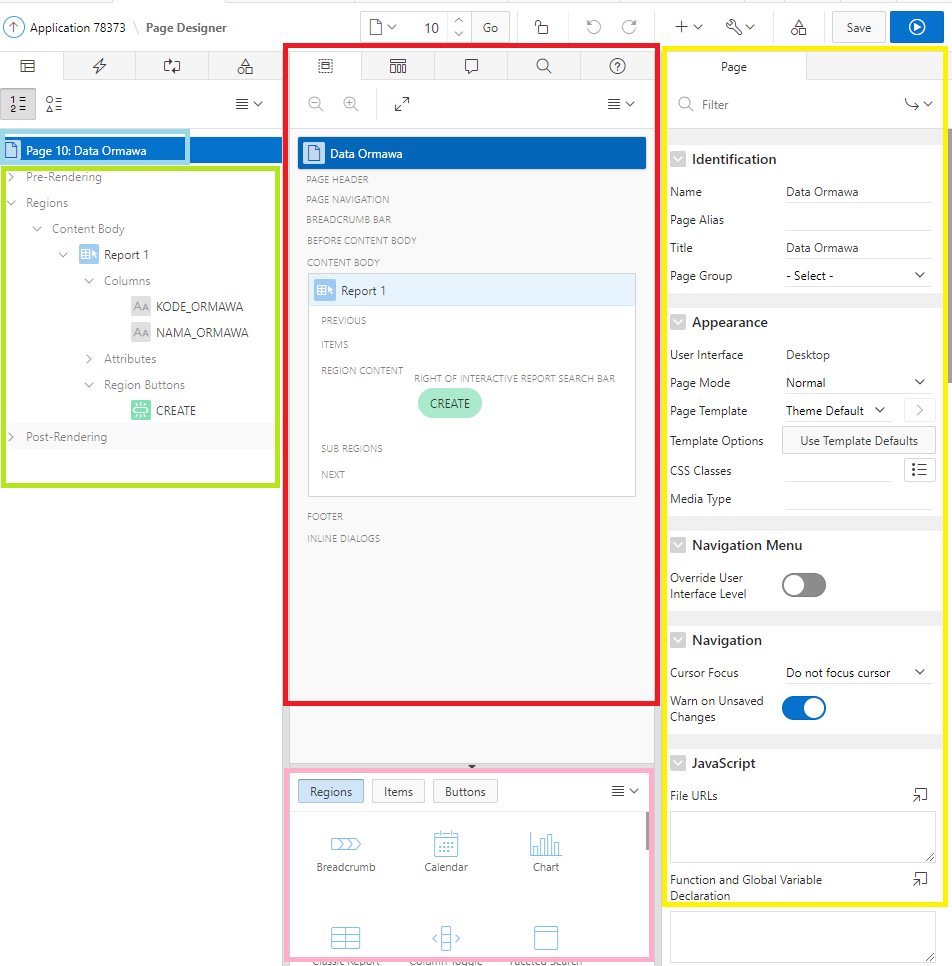
\includegraphics[scale=0.45]{figures/halaman_page_designer.png}
        \caption{\textit{Halaman Edit Page Designer}}
        \end{center}
        Deskripsi
        \begin{itemize}
            \item  HIJAU = Adalah list dari isi page tersebut yang berisi tabel report dari ORMAWA
            \item  MERAH = Adalah isi dari halaman yang akan ditampilkan anda bisa membuat segala macam atribut seperti kalender,box,tombol,chart,dll tinggal seret dari kolom yang ditandai dengan warna merah jambu
        \end{itemize}
        \end{figure}
    
        \begin{figure}[!htbp]
        \begin{itemize}
            \item MERAH JAMBU = adalah isi dari atribut seperti button,text,chart,kalender,breadcumb,bar,dll
            \item KUNING = adalah isi dari page anda bisa mengatunya pada tampilan ini
        \end{itemize}
        \item[9]Sementara pada halaman FORM
        \begin{center}
        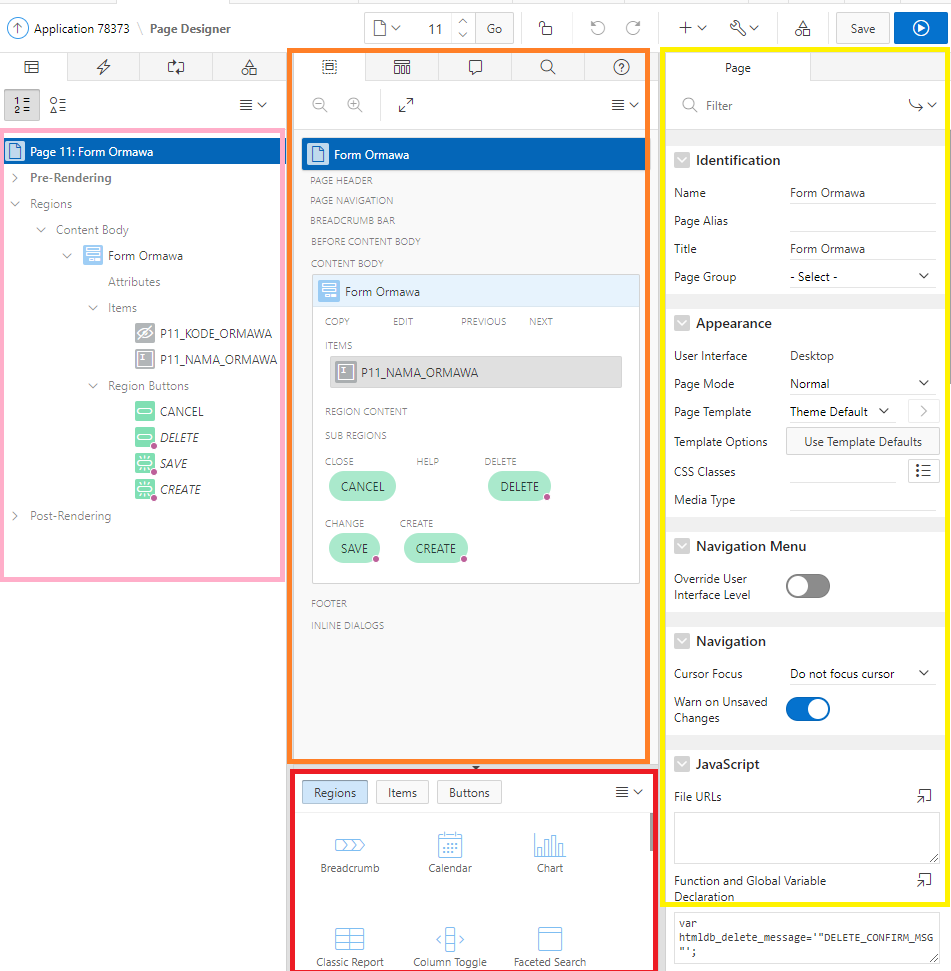
\includegraphics[scale=0.45]{figures/halaman_page_designer_form.png}
        \caption{\textit{Halaman Utama Apex}}
        \end{center}
         \begin{itemize}
            \item  Merah Jambu = Adalah list dari isi page tersebut yang berisi form untuk tabel ORMAWA
            \item  Oranye = Adalah isi dari halaman yang akan ditampilkan anda bisa membuat segala macam atribut seperti kalender,box,tombol,chart,dll tinggal seret dari kolom yang ditandai dengan warna merah jambu
        \end{itemize}
        \end{figure}
        \begin{itemize}
            \item  MERAH = adalah isi dari atribut seperti button,text,chart,kalender,breadcumb,bar,dll.
            \item  KUNING = adalah isi dari page anda bisa mengaturnya segala macam mulai dari proses identifikasi sampai yang lain pada tampilan ini. 
        \end{itemize}
\end{itemize}


